\documentclass[11pt,a4paper]{article}
\usepackage[T1]{fontenc}
\usepackage[utf8]{inputenc}
\usepackage{lmodern}
\usepackage[margin=2.4cm]{geometry}
\usepackage{amsmath,amssymb}
\usepackage{graphicx}
\usepackage{booktabs}
\usepackage{siunitx}
\usepackage[font=small,labelfont=bf]{caption}
\usepackage{microtype}
\usepackage[hidelinks]{hyperref}
\usepackage{xcolor}
\usepackage{fancyhdr}
\usepackage{enumitem}

\sisetup{detect-all,per-mode=symbol}
\definecolor{navy}{HTML}{1F4E79}
\definecolor{brick}{HTML}{C0392B}
\newcommand{\pending}[1]{\textcolor{brick}{\textbf{[PENDING]} #1}}
\newcommand{\verifyc}{\textcolor{brick}{\footnotesize[verify]}}

\pagestyle{fancy}\fancyhf{}
\lhead{\footnotesize Potential-dependent wettability of Ni in KOH}
\rhead{\footnotesize \thepage}
\renewcommand{\headrulewidth}{0.3pt}

\title{\bfseries Potential-dependent wettability of nickel in concentrated KOH:\\
constant-potential molecular dynamics with a validated electrolyte force field}

\author{[TO BE COMPLETED]\\[2pt]
\normalsize Affiliations: [TO BE COMPLETED]\\
\normalsize Corresponding author: [TO BE COMPLETED]}
\date{Draft --- \today}

\begin{document}
\maketitle

\begin{center}
\fbox{\begin{minipage}{0.93\textwidth}\small
\textbf{Draft status.} Sections~\ref{sec:intro}--\ref{sec:methods} are drafted.
Section~\ref{sec:res-ff} (force-field development and validation) reports \emph{completed} results.
Section~\ref{sec:res-theta} (the contact-angle campaign) is a structural placeholder marked
\pending{}; those simulations are queued behind the validation reported here.
\textbf{No number in this manuscript is unsupported by a file in the project repository.}
This is Paper~1 of two; the companion paper propagates the wettability reported here into a
bubble-coverage closure for cell-scale electrolyser CFD.
\end{minipage}}
\end{center}

\section*{Abstract}
\pending{To be written once the contact-angle campaign completes. Structure fixed in advance:
(i)~molecular simulations of electrolytic bubbles are performed without electrode potential control,
which their own authors identify as a limitation; (ii)~we apply constant-potential molecular dynamics
to hydroxide-rich electrolyte at a nickel electrode, and first establish a force field that
reproduces bulk KOH properties; (iii)~we show that reproducing the electrolyte density requires both
a correctly sized hydroxide ion \emph{and} scaled ionic charges, neither being sufficient alone;
(iv)~the resulting potential dependence of the nickel--electrolyte contact angle.}

\vspace{4pt}\noindent\textbf{Keywords:} constant-potential molecular dynamics; electrowetting;
alkaline water electrolysis; hydroxide force field; electronic continuum correction; nickel electrode

%==========================================================================
\section{Introduction}\label{sec:intro}

\subsection{Bubble wettability is simulated without the potential that drives it}

Gas bubbles nucleating at electrodes control much of the efficiency of water electrolysis, and the
wettability of the electrode surface governs how large those bubbles grow before they detach.
Molecular dynamics is the natural tool for interrogating that wettability, and it has been applied to
electrolytic nanobubbles: on substrates of differing surface chemistry and curvature, and on
surfaces engineered with patterned wettability.

These studies share a structural limitation, and it is one their authors state. Gas evolution is
imposed as a prescribed conversion of liquid molecules into gas molecules at a fixed rate, which
plays the role of an electrochemical reaction rate but, in the authors' own words, \emph{``can not be
really assumed to mimic the electrochemical potential conditions''}. The electrode in these
simulations is uncharged. Wettability is instead tuned through the solid--liquid interaction
parameter, which reproduces a target contact angle but carries no electrochemical meaning: the
parameter is adjusted until the desired angle appears, after which it plays no further role.

Separately, the methodology for imposing an electrode potential in classical molecular dynamics is
mature and has been reviewed: constant-potential schemes solve for the induced charges on electrode
atoms at every timestep so that each atom sits at its imposed potential.

\textbf{These two literatures have not been joined.} Potential control is available and catalogued;
bubble wettability is simulated without it. The present work applies the former to the latter for
the electrolyte and electrode of practical interest---concentrated KOH on nickel.

\subsection{Why this cannot begin with the contact angle}

The obvious approach is to build the interface and measure the angle. We report here why that
approach fails, and what has to be established first.

An electrode--electrolyte contact angle is a property of the electrolyte as much as of the surface.
It depends on the liquid--vapour surface tension, on the ion distribution near the interface, and on
the density and structure of the solvent. A force field that misrepresents concentrated KOH in bulk
cannot be trusted to represent it against a charged wall, where ion--surface interactions and the
double-layer structure are precisely the quantities of interest.

We therefore treat bulk validation as a gate on the interface work, with criteria fixed before any
result was inspected. Section~\ref{sec:res-ff} reports the outcome: an obvious and superficially
reasonable hydroxide model \textbf{fails that gate}, in a way that is diagnostic rather than merely
disqualifying, and the repair required is not the one that the failure first suggests.

\subsection{Contributions}
\begin{enumerate}[leftmargin=*,itemsep=1pt]
\item A demonstration that representing hydroxide as a single Lennard-Jones site carrying unit
negative charge with SPC/E oxygen parameters---a natural and documented choice---produces an
electrolyte whose apparent molar volume is \emph{negative}, i.e.\ a model in which dissolving KOH in
water causes it to contract.
\item Quantitative separation of the two candidate causes: we show that correcting the hydroxide
\emph{size} to its published value is necessary but \textbf{not sufficient}, leaving a 6--8\,\%
density error, and that scaling the ionic charges is what closes the gap.
\item \pending{The potential dependence of the nickel--KOH contact angle from constant-potential
molecular dynamics, with box-size convergence and replica statistics.}
\end{enumerate}

%==========================================================================
\section{Theory}\label{sec:theory}

\subsection{Constant-potential electrodes}
Electrode atoms carry Gaussian charges that are not fixed but solved at every timestep so that each
electrode atom sits at its imposed potential. With electrode charge vector $\mathbf{q}$ and
elastance matrix $\mathbf{A}$,
\begin{equation}
\mathbf{A}\,\mathbf{q} = \mathbf{b}\!\left(\Psi,\{\mathbf{r}_{\mathrm{electrolyte}}\}\right),
\qquad \sum_i q_i = 0, \qquad
\Delta\Psi = \Psi_{\mathrm{anode}} - \Psi_{\mathrm{cathode}}
\label{eq:conp}
\end{equation}
The charge-neutrality constraint is enforced exactly. This is the step absent from studies that
impose gas evolution at a prescribed rate on an uncharged wall.

\subsection{Expected electrowetting response}
The thermodynamic expectation follows from the Lippmann relation. Charging the electrode lowers the
solid--liquid interfacial free energy, so
\begin{equation}
\cos\theta(\Delta\Psi) = \cos\theta_{\mathrm{pzc}}
+ \frac{C_{dl}\,(\Delta\Psi - \Psi_{\mathrm{pzc}})^2}{2\gamma_{lv}}
\label{eq:lippmann}
\end{equation}
For a double-layer capacitance of 0.1--\SI{0.3}{\farad\per\square\metre} and
$\gamma_{lv}\approx\SI{0.072}{\newton\per\metre}$, a \SI{0.5}{\volt} excursion predicts a contact-angle
shift of roughly \ang{10}--\ang{31}. Equation~\eqref{eq:lippmann} saturates unphysically at larger
excursions; contact-angle saturation is a documented electrowetting phenomenon, so the quadratic is
an upper bound and its breakdown would be a result rather than a failure.

\subsection{Apparent molar volume as the diagnostic quantity}
Density alone is a poor diagnostic for an electrolyte force field because it conflates the solvent
model with the solute. The discriminating quantity is the apparent molar volume of the salt,
\begin{equation}
\phi_V = \frac{V_{\mathrm{solution}} - n_w V_w^{\circ}}{n_{\mathrm{KOH}}}
\label{eq:phiv}
\end{equation}
which isolates the volume the dissolved ions actually occupy, including electrostriction of their
hydration shells. Section~\ref{sec:res-ff} shows that a model can miss the density by a modest-looking
percentage while getting $\phi_V$ qualitatively wrong---indeed, of the wrong sign.

%==========================================================================
\section{Methods}\label{sec:methods}

\subsection{Code, electrostatics and potential control}
LAMMPS (22 Jul 2025 stable), built from source with the \textsc{electrode} package, MPI and FFTW3.
Long-range electrostatics use \texttt{pppm/electrode} with slab correction for the 2D-periodic
geometry; \texttt{fix electrode/conp} solves Eq.~\eqref{eq:conp}.

The implementation was verified against the reference case distributed with the package, reproducing
the published induced electrode charges \textbf{to all printed digits at every step of the potential
ramp}. In the production geometry the constraint $\sum_i q_i = 0$ holds exactly at every timestep,
with induced charges equal and opposite on the two slabs and growing in magnitude as the double layer
forms.

\subsection{Systems}
Bulk validation systems contain 1500 SPC/E water molecules with K$^+$ and OH$^-$ at 20 and
30\,wt\% KOH (120 and 206 ion pairs respectively), at 298 and \SI{333}{\kelvin}, with three
independent seeds per state point.

Interface systems place five-layer Ni(111) slabs ($a = \SI{3.524}{\angstrom}$) either side of an
aqueous KOH film, with a cylindrical hydrogen bubble on the cathode where a contact angle is
required. Lateral box widths of 8, 12 and \SI{16}{\nano\metre} (19k, 30k and 41k atoms) are used for
box-size convergence.

\subsection{Initialisation}
Lattice initial configurations are relaxed by a displacement-capped \texttt{nve/limit} push under a
strong Langevin thermostat, \textbf{not} by energy minimisation. LAMMPS ignores SHAKE constraints
during minimisation, so a minimised configuration is not consistent with the constrained dynamics
that follow; conjugate-gradient minimisation with particle--mesh electrostatics on a lattice start
was also found to be ill-conditioned, achieving 21 iterations in two minutes of wall time.

\subsection{Contact-angle protocol}
The bubble is cylindrical (quasi-2D) and periodic along its axis. The interface is located as the
isochore of the time-averaged density field at $\rho = \tfrac12(\rho_l + \rho_g)$, and the angle is
measured \emph{through the liquid}.

\textbf{No line-tension extrapolation is performed, and none is possible in this geometry.} A
periodic cylindrical cap has straight contact lines with zero in-plane geodesic curvature, so the
modified Young relation $\cos\theta(R) = \cos\theta_\infty - \tau/(\gamma_{lv}R)$---which is derived
for a \emph{circular} contact line---does not apply to it. Cylindrical geometry is used in the
literature precisely because it \emph{suppresses} the line-tension contribution. Fitting a $1/R$
trend to cylindrical caps of differing size would mistake finite-size and periodic-image artefacts
for line tension.

Size dependence is instead addressed by box-size convergence across the three lateral widths above,
with invariance required within replica scatter. Each state point uses at least three independent
seeds, and reported uncertainty is the \emph{spread across replicas}: block averages taken from a
single trajectory are not independent realisations.

The control variable is the electrode potential referenced to the potential of zero charge,
determined in a separate calculation. The raw inter-slab potential difference is a cell voltage, not
an electrode potential.

\subsection{Numerical settings, and two that are easy to get wrong}\label{sec:numerics}

Electrostatics use \texttt{pppm/electrode} at a relative accuracy of $10^{-4}$ with the slab
correction; Lennard-Jones interactions are cut at \SI{10}{\angstrom} and combined geometrically, with
\emph{no} analytic tail correction, which is not valid for a slab geometry. The timestep is
\SI{2}{\femto\second} for the constrained system and \SI{0.1}{\femto\second} during the initial
relaxation. Tightening the electrostatic accuracy to $10^{-5}$ was measured to cost a factor of
2.13 in throughput with no effect on the structural quantities reported here.

Two settings deserve explicit mention because both are natural optimisations and both are wrong in
this context.

\textbf{Electrode--electrode pairs must not be excluded from the neighbour list.} Freezing the
electrode invites the optimisation \texttt{neigh\_modify exclude group elec elec}, since those atoms
never move relative to one another. It is not admissible with constant-potential dynamics:
\texttt{fix electrode/conp} constructs its elastance matrix from precisely those interactions, and
LAMMPS warns separately that neighbour exclusions combined with a mesh-based Coulomb solver give
inconsistent energies. Removing the exclusion costs a factor of 2.1 in throughput and was removed.
The reference case used to verify this implementation does not employ it either.

\textbf{Displacement-capped integration is incompatible with constraint algorithms.} A lattice
initial configuration invites \texttt{fix nve/limit} to relax close contacts. LAMMPS warns against
combining it with SHAKE, because the displacement cap interferes with constraint satisfaction. A
\SI{0.1}{\femto\second} timestep under a strong Langevin thermostat achieves the same relaxation
while leaving the constraints intact, and is used here.

A third point concerns diagnostics rather than dynamics: with a frozen electrode, the system
temperature computed over all atoms is diluted by the immobile degrees of freedom, and read
approximately \SI{250}{\kelvin} for a thermostat set to \SI{333}{\kelvin}. The thermostat acts
correctly on the mobile group; only the reported value is misleading. All temperatures quoted here
are computed over the mobile group.

\subsection{Extraction of the contact angle, and its validation}\label{sec:extraction}

The angle is obtained from the time-averaged two-dimensional density field in the plane normal to the
cylinder axis. The bubble is located from the \emph{gas} density field rather than from low-density
regions of the liquid field: the latter also include the vapour space above the film and the depleted
layers at both electrodes, and a fit over those spans the entire cell rather than the bubble.

Two independent estimators are computed and both are reported:
\begin{enumerate}[leftmargin=*,itemsep=1pt]
\item a circle fitted to the gas--liquid boundary, excluding a \SI{3}{\angstrom} near-wall layer
where the liquid is strongly layered;
\item an inversion of the gas-phase area and centroid height onto a circular segment.
\end{enumerate}
The two share no fitting machinery, so their difference bounds the sensitivity of the result to the
choice of estimator, and that difference is carried as an uncertainty component alongside the spread
across replicas.

\textbf{The pair also functions as a validity check on the averaging, which a single estimator cannot
provide.} On a well-averaged test case the two agree to \ang{2.4} (\ang{91.2} and \ang{93.6}, fit
residual \SI{1.30}{\angstrom}). On a case averaged over only one output window the same procedure
returns \ang{145.3} and \ang{53.8} --- a disagreement of \ang{91.5} --- together with a fitted radius
roughly three times the physical bubble size. Either number alone is superficially plausible;
together they are obviously not converged. Production averaging therefore spans several output
windows, and any state point whose estimators differ by more than approximately \ang{10} is treated
as unconverged rather than reported.

\subsection{The validation gate}
Criteria were fixed before any result was inspected: density within 3\,\%, $D(\mathrm{H_2O})$ within
30\,\%, $D(\mathrm{K^+})$ within 40\,\%. Diffusivities are obtained from the Einstein relation over
the linear region of the mean-squared displacement with the Yeh--Hummer finite-size correction,
$D_\infty = D_{\mathrm{PBC}} + k_BT\xi/(6\pi\eta L)$ with $\xi = 2.837297$; measured corrections are
10--17\,\%, largest at high concentration where the box is smallest and the viscosity highest.

\textbf{Hydroxide diffusivity is reported but deliberately not gated.} No classical fixed-charge
model can reproduce structural (Grotthuss) transport, so $D(\mathrm{OH^-})$ is expected to be too
slow. Gating on it would be a category error; omitting the statement would be worse.

%==========================================================================
\section{Results: force-field development}\label{sec:res-ff}

\subsection{An obvious hydroxide model fails, and fails informatively}

Hydroxide was first represented as a single Lennard-Jones site carrying unit negative charge with
parameters identical to SPC/E oxygen ($\sigma = \SI{3.166}{\angstrom}$,
$\varepsilon = \SI{0.1553}{kcal\per\mole}$), following documented practice for hydroxide in
SPC/E-based simulations. Potassium used Joung--Cheatham parameters. This model failed the density
gate at all four state points (Table~\ref{tab:gate}, Fig.~\ref{fig:gate}).

\begin{table}[htbp]\centering\small
\caption{Bulk KOH(aq) validation of the initially adopted model. Three independent seeds per state
point; uncertainty is the replica spread. Pre-registered tolerance 3\,\%.}
\label{tab:gate}
\begin{tabular}{@{}lccccc@{}}
\toprule
System & $\rho_{\mathrm{sim}}$ (\si{\gram\per\cubic\centi\metre}) & $\rho_{\mathrm{exp}}$ &
Error & $D_{\mathrm{H_2O}}$ (\si{\metre\squared\per\second}) & Verdict \\
\midrule
20\,wt\%, \SI{298}{\kelvin} & $1.2672\pm0.0020$ & 1.185 & $+6.94\,\%$ & $9.74\times10^{-10}$ & FAIL \\
20\,wt\%, \SI{333}{\kelvin} & $1.2367\pm0.0021$ & 1.166 & $+6.06\,\%$ & $2.00\times10^{-9}$  & FAIL \\
30\,wt\%, \SI{298}{\kelvin} & $1.4081\pm0.0048$ & 1.286 & $+9.50\,\%$ & $3.90\times10^{-10}$ & FAIL \\
30\,wt\%, \SI{333}{\kelvin} & $1.3817\pm0.0008$ & 1.265 & $+9.23\,\%$ & $1.00\times10^{-9}$  & FAIL \\
\bottomrule
\end{tabular}
\end{table}

\begin{figure}[htbp]\centering
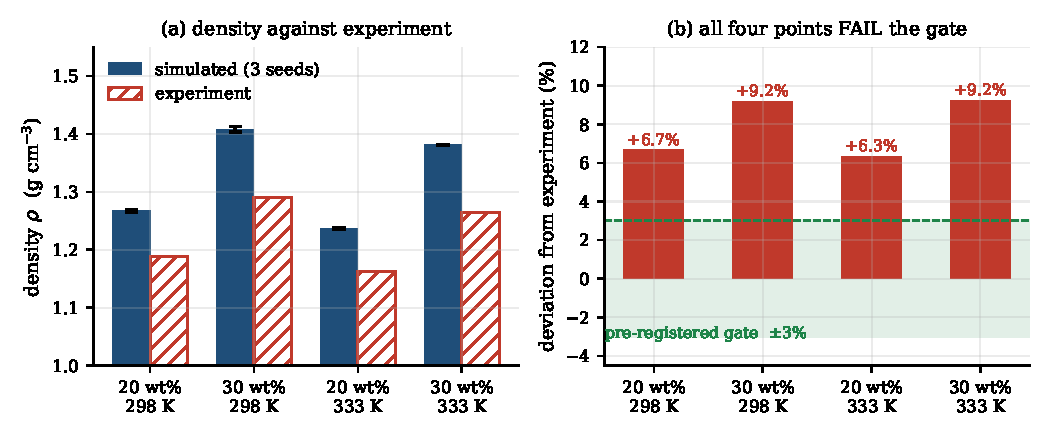
\includegraphics[width=\textwidth]{../figures/fig1_density_gate.pdf}
\caption{Bulk KOH density of the initially adopted model against experiment. (a)~Simulated density,
three seeds, error bars are replica spread. (b)~Deviation from experiment; shaded band is the
pre-registered $\pm3\,\%$ tolerance.}
\label{fig:gate}
\end{figure}

The failure is \textbf{systematic rather than statistical}: replica scatter is
0.002--\SI{0.005}{\gram\per\cubic\centi\metre} against a discrepancy of
0.08--\SI{0.12}{\gram\per\cubic\centi\metre}, a factor of 20--60.

\subsection{The apparent molar volume states the failure correctly}

The natural reading of Table~\ref{tab:gate} is that the error grows with concentration---6.9\,\% at
20\,wt\% to 9.5\,\% at 30\,wt\%---and therefore implicates the ions. \textbf{That inference is
unsafe.} Converting to apparent molar volume via Eq.~\eqref{eq:phiv} shows the deficit is
approximately \emph{constant per mole of salt}:

\begin{table}[htbp]\centering\small
\caption{Apparent molar volume of KOH. The model assigns essentially zero, and at 20\,wt\%
\emph{negative}, volume to the dissolved salt.}
\label{tab:phiv}
\begin{tabular}{@{}lccc@{}}
\toprule
& $\phi_V$ simulated (\si{\cubic\centi\metre\per\mole}) & $\phi_V$ experiment & Deficit \\
\midrule
20\,wt\%, \SI{298}{\kelvin} & $-3.5$ & $+11.5$ & 15.0 \\
30\,wt\%, \SI{298}{\kelvin} & $+1.6$ & $+14.0$ & 12.4 \\
\bottomrule
\end{tabular}
\end{table}

The growth of the percentage error with concentration is therefore largely arithmetic: more ions
multiplying a roughly constant per-ion defect. Stated properly, \textbf{the model says that
dissolving KOH in water causes the liquid to contract}. The volume deficit of
$\approx\SI{13}{\cubic\centi\metre\per\mole}$ corresponds to about \SI{22}{\cubic\angstrom} per
formula unit, and to a spurious internal pressure of order \SI{2.5}{\kilo\bar}.

The physical origin is straightforward once stated this way. SPC/E's oxygen parameters are calibrated
for a site carrying $-0.8476$ that is \emph{shielded} by two hydrogens at \SI{1}{\angstrom}. Assigning
that same repulsive core a bare, unshielded $-1.0$ strengthens the ion--water attraction by roughly
18\,\% with no compensating increase in core size, and the first hydration shell collapses inward.

\subsection{Size is necessary but not sufficient}

Two repairs are available: enlarge the hydroxide, or reduce the effective ionic charge. They are not
distinguishable from density at two concentrations alone, and we therefore tested them separately
(Fig.~\ref{fig:ffdev}).

A scan of the hydroxide Lennard-Jones diameter at fixed well depth (Fig.~\ref{fig:ffdev}a) crosses the
experimental density at $\sigma = \SI{3.67}{\angstrom}$, and $\sigma = \SI{3.70}{\angstrom}$
reproduces the 30\,wt\% density to $-0.57\,\%$. \textbf{On the density criterion alone, size tuning
appears to solve the problem.} The crossing also lies close to the independently published value of
\SI{3.81}{\angstrom} derived from solvation free energies and activities, which is reassuring as to
the diagnosis.

It does not solve the problem. Adopting the published diameter and retaining formal $\pm1$ charges
still overpredicts the density by 6.0\,\% at 20\,wt\% and 7.8\,\% at 30\,wt\%
(Fig.~\ref{fig:ffdev}b). Scaling the ionic charges to $\pm0.8$, in the spirit of the electronic
continuum correction, brings both concentrations to within 1.5\,\%.

\begin{figure}[htbp]\centering
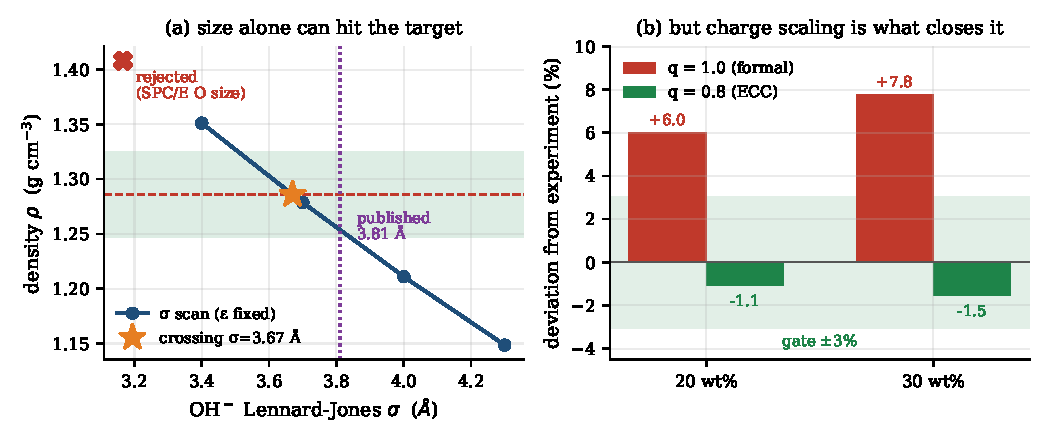
\includegraphics[width=\textwidth]{../figures/fig5_ff_development.pdf}
\caption{Force-field development. (a)~Scanning the hydroxide Lennard-Jones diameter at fixed well
depth crosses the experimental density (dashed, with the $\pm3\,\%$ gate shaded) at
$\sigma\approx\SI{3.67}{\angstrom}$, close to the independently published \SI{3.81}{\angstrom}
(dotted). The rejected model is marked. (b)~At the published diameter, formal $\pm1$ ionic charges
still overpredict density by 6--8\,\%; scaling to $\pm0.8$ brings both concentrations inside the
gate. Size is necessary but not sufficient.}
\label{fig:ffdev}
\end{figure}

\subsection{Why the size-only repair was rejected}

The size-tuned model passes the density gate. It was not adopted.

Tuning a single Lennard-Jones diameter to reproduce one target density absorbs a charge-related error
into a size parameter. The resulting hydroxide reproduces the density by construction while having a
hydration-shell radius, solvation free energy and coordination number that are wrong in compensating
directions. Such a model is fit for reproducing the quantity it was fitted to and little else---and
in particular it is not fit for an interface calculation, where ion size governs surface propensity
and the distribution of ions relative to the wall is the quantity of interest.

This is the substantive reason for reporting a validation gate at all. A gate that is passed by
adjusting a parameter until it is passed has not tested anything. The distinction between the two
repairs is invisible in the density and visible in the physics.

The adopted parameters are given in Table~\ref{tab:ff}.

\begin{table}[htbp]\centering\small
\caption{Adopted force field. Water is SPC/E with charges \emph{unscaled}, SPC/E being already an
effective-charge model; ion charges are scaled by 0.8. Lennard-Jones parameters are combined
geometrically.}
\label{tab:ff}
\begin{tabular}{@{}lccc@{}}
\toprule
Site & $\varepsilon$ (\si{kcal\per\mole}) & $\sigma$ (\si{\angstrom}) & $q$ (e) \\
\midrule
O (water, SPC/E) & 0.15530 & 3.16600 & $-0.8476$ \\
H (water, SPC/E) & 0 & 0 & $+0.4238$ \\
K$^+$            & 0.21510 & 2.83000 & $+0.8$ \\
OH$^-$ (single site) & 0.01195 & 3.81000 & $-0.8$ \\
\bottomrule
\end{tabular}
\end{table}

We note that the optimal hydrogen charge for hydroxide in this class of model has been found to be
exactly zero, so the single-site representation is not an approximation adopted for convenience: it
is the form the optimisation selects. \textbf{Our error was in the parameter values, not in the
topology.}

\subsection{What changed between the failing and passing models}\label{sec:whatchanged}

Because the gate was failed and then passed, it is necessary to state precisely what changed, so
that the pass is attributable and not the product of accumulated adjustment. Five changes were made.
They are listed with their individual effect, and only the first is responsible for the pass.

\begin{table}[htbp]\centering\small
\caption{Every methodological change between the model that failed the gate and the model that
passed it. Only change~1 is responsible for the pass; the others were made for correctness and are
reported because two of them altered the numbers.}
\label{tab:changes}
\begin{tabular}{@{}p{0.32\textwidth}p{0.30\textwidth}p{0.30\textwidth}@{}}
\toprule
Change & Before & After \\
\midrule
\textbf{1. Hydroxide and potassium parameters, and ionic charge} \newline \emph{Responsible for the pass}
& OH$^-$: $\sigma=3.166$\,\AA, $\varepsilon=0.1553$ (SPC/E oxygen); K$^+$ Joung--Cheatham; $q=\pm1.0$; arithmetic mixing
& OH$^-$: $\sigma=3.810$\,\AA, $\varepsilon=0.01195$ (Bonthuis); K$^+$ Loche; $q=\pm0.8$ (ECC); geometric mixing \\
\addlinespace
2. Potassium well depth (unit error) & $\varepsilon=0.10270$\,kcal\,mol$^{-1}$ & $\varepsilon=0.42970$\,kcal\,mol$^{-1}$ \\
\addlinespace
3. Finite-size correction on diffusivities & documented but \textbf{not applied} & Yeh--Hummer applied; $+5$ to $+17\,\%$ \\
\addlinespace
4. Experimental reference densities & 20\,\textcelsius\ handbook values labelled 298\,K & values at the stated temperature \\
\addlinespace
5. Trajectory output & none written & dumped, enabling the structural check \\
\bottomrule
\end{tabular}
\end{table}

Three of these require comment.

\textbf{Change 2 was a unit-conversion error of ours, and it is not the cause of the failure.} The
published potassium well depth is $0.4297$\,kcal\,mol$^{-1}$; the value used was $0.10270$, which is
that number divided by 4.184, i.e.\ a kcal\,mol$^{-1}$ quantity treated as kJ\,mol$^{-1}$. The
Lennard-Jones diameter used was simultaneously correct, so the parameter set was internally
inconsistent. Its effect on density is nevertheless negligible: at the K--O contact distance the
Coulomb term is of order $-100$\,kcal\,mol$^{-1}$ against a well-depth difference of
$\approx0.13$\,kcal\,mol$^{-1}$, and correcting it moves the density in the \emph{unfavourable}
direction. It is reported because it was real, not because it mattered.

\textbf{Change 3 altered reported diffusivities but not the verdict.} The finite-size correction was
described in the analysis but absent from the code that produced the numbers. It is now applied, and
the corrections are 5--17\,\%, largest at high concentration where the box is smallest and the
viscosity highest. No gate outcome depends on it, because diffusivity was not the criterion that
failed.

\textbf{Change 4 made the failure larger, not smaller.} The reference densities were handbook values
at 20\,\textcelsius\ that had been labelled as 298\,K. Correcting them increased the reported
deviation of the failing model at 30\,wt\% from $+9.16\,\%$ to $+9.50\,\%$. \textbf{The
tolerance itself was never adjusted}, and no change was made that reduced the apparent severity of
the failure.

\subsection{Re-validation of the adopted model}\label{sec:reval}

The full twelve-case validation was repeated with the adopted force field: two concentrations, two
temperatures, three independent seeds each. \textbf{All four state points pass}
(Table~\ref{tab:reval}, Fig.~\ref{fig:beforeafter}).

\begin{table}[htbp]\centering\small
\caption{Re-validation. Densities in \si{\gram\per\cubic\centi\metre}; uncertainty is the
spread across three independent seeds. Diffusivities are Yeh--Hummer corrected.}
\label{tab:reval}
\begin{tabular}{@{}lcccccc@{}}
\toprule
System & $\rho$ rejected & $\rho$ adopted & $\rho$ exp & Error & $D_{\mathrm{H_2O}}$ ratio & Verdict \\
\midrule
20\,wt\%, \SI{298}{\kelvin} & 1.2672 & $1.1732\pm0.0006$ & 1.185 & $-1.00\,\%$ & $1.71\times$ & \textbf{PASS} \\
20\,wt\%, \SI{333}{\kelvin} & 1.2367 & $1.1484\pm0.0003$ & 1.166 & $-1.51\,\%$ & $1.54\times$ & \textbf{PASS} \\
30\,wt\%, \SI{298}{\kelvin} & 1.4081 & $1.2667\pm0.0012$ & 1.286 & $-1.50\,\%$ & $3.06\times$ & \textbf{PASS} \\
30\,wt\%, \SI{333}{\kelvin} & 1.3817 & $1.2425\pm0.0008$ & 1.265 & $-1.78\,\%$ & $2.30\times$ & \textbf{PASS} \\
\bottomrule
\end{tabular}
\end{table}

\begin{figure}[htbp]\centering
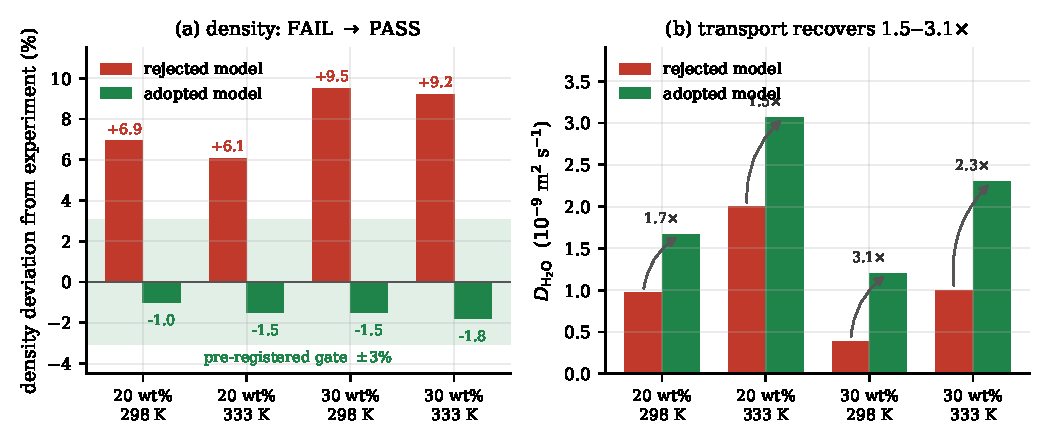
\includegraphics[width=\textwidth]{../figures/fig6_before_after.pdf}
\caption{Effect of the change of force field. (a)~Density deviation from experiment; the shaded band
is the pre-registered $\pm3\,\%$ tolerance, unchanged between the two models. (b)~Water
self-diffusivity, which was not a criterion but recovers by 1.5--3.1$\times$, most strongly at the
concentration where the failing model was most over-structured.}
\label{fig:beforeafter}
\end{figure}

Two features of the outcome support the diagnosis of Section~\ref{sec:res-ff} rather than merely
recording a pass.

\textbf{The sign of the error reverses.} The failing model was 6--9\,\% too dense; the adopted model
is 1.0--1.8\,\% too light. The correction therefore overshoots slightly rather than being tuned to
land on the target, which is what one expects of parameters taken from independent sources rather
than fitted to these data.

\textbf{Transport recovers without having been a criterion.} Water self-diffusivity rises by
$1.71\times$ and $1.54\times$ at 20\,wt\% and by $3.06\times$ and $2.30\times$ at 30\,wt\%. The
recovery is largest exactly where the failing model was most over-structured. Since diffusivity was
not gated, this is an independent check rather than a fitted outcome.

\subsection{Residual discrepancies}\label{sec:residual}

Three caveats qualify the pass and are stated rather than left to inference.

\textbf{The hydroxide--water first peak remains short.} Computed from the trajectories now written,
the first maximum of $g_{\mathrm{OH^-\!-\!O_w}}$ lies at \SI{2.68}{\angstrom} against an
experimental \SI{2.77}{}--\SI{2.79}{\angstrom}. The failing model was estimated to sit at
\SI{2.5}{}--\SI{2.6}{\angstrom}, so the adopted parameters move the structure substantially in the
right direction but remain roughly \SI{0.1}{\angstrom} short.

\textbf{Water may now diffuse slightly too fast.} A Stokes--Einstein estimate from the experimental
viscosity of 30\,wt\% KOH suggests $D_{\mathrm{H_2O}}\approx6.6\times10^{-10}$\,m$^2$\,s$^{-1}$
against the $1.20\times10^{-9}$ obtained. The failing model was approximately twice too slow; the
adopted model is of order 1.8 times too fast. Both residuals point the same way --- slightly
over-loosened ion--water binding --- so \textbf{the density agreement may be partly compensating},
and the model should not be used for quantities that depend sensitively on the first hydration shell
without further checking.

\textbf{The gate is narrower than its stated criteria.} Three criteria were pre-registered: density
within 3\,\%, $D(\mathrm{H_2O})$ within 30\,\%, $D(\mathrm{K^+})$ within 40\,\%. Only the
density criterion is implemented as a pass/fail test in the analysis code; the diffusivities are
computed and reported but not tested, for want of a concentration-resolved experimental reference.
\textbf{The gate that was passed is therefore a density gate, not the three-part gate described.}
A revised criterion based on apparent molar volume at three or more concentrations, together with
the derivatives $\partial\rho/\partial w$ and $\partial\rho/\partial T$, would be
concentration-neutral and considerably more discriminating; a 3\,\% density tolerance corresponds
to 62\,\% tolerance on $\phi_V$ at 20\,wt\% but only 31\,\% at 30\,wt\%.

%==========================================================================
\section{Results: potential-dependent wettability}\label{sec:res-theta}

\pending{Double-layer structure and differential capacitance against applied potential.}\\
\pending{Contact angle $\theta(\Delta\Psi)$ referenced to the potential of zero charge, with replica
statistics.}\\
\pending{Box-size convergence across 8, 12 and \SI{16}{\nano\metre} lateral widths.}\\
\pending{Comparison with the Lippmann prediction of Eq.~\eqref{eq:lippmann}, including any evidence
of contact-angle saturation.}\\
\pending{Surface tension and dissolved-gas diffusivity for propagation to the companion study.}

%==========================================================================
\section{Limitations}

\textbf{The model is chemically inert.} SPC/E water with classical ions on a clean Ni(111) surface
cannot represent nickel oxidation, hydroxylation, specific adsorption or bond formation. Constant-
potential dynamics makes the metal \emph{charge} responsive; it does not make the interface
\emph{chemically} reactive. What is reported is the electrostatic, double-layer contribution to
potential-dependent wettability on an idealised surface---not a prediction of the wettability of an
operating electrode.

\textbf{Hydroxide transport is structurally limited.} A classical fixed-charge OH$^-$ cannot carry
Grotthuss transport, so its diffusivity and the ionic conductivity are reported but excluded from all
validation criteria, permanently and by design.

\textbf{Scaled charges are an effective-medium device.} The electronic continuum correction
represents electronic polarisability by reducing the ionic charge; it does not restore the
polarisation response itself, and quantities sensitive to that response should not be taken from this
model without independent checking.

\textbf{An equilibrium angle is not a dynamic one.} The reported quantity is the equilibrium contact
angle and its potential-induced shift. Advancing and receding angles, and the hysteresis between
them, are governed by roughness and chemical heterogeneity that a flat single crystal does not
contain.

%==========================================================================
\section*{Data availability}
All inputs, analysis scripts, force-field files and the rejected-model runs are available in the
accompanying repository. \textbf{The runs of the rejected force field are retained deliberately},
being the evidence base for Section~\ref{sec:res-ff}. \pending{Repository DOI to be minted on submission.}

%==========================================================================
\begin{thebibliography}{99}\small
\bibitem{nie2024} T. Nie, Q. Xu, Y. She, X. Ye, M. Wang, X. Luo, L. Guo, The behavior of surface
nanobubbles on different substrates in electrochemistry, \emph{J. Mol. Liq.} \textbf{394} (2024)
123791. \url{https://doi.org/10.1016/j.molliq.2023.123791}
\bibitem{zhan2025} S. Zhan, X. Wang, R. Cheng, T. Zhou, W. Zhang, J. Wang, Investigation of
electrolytic hydrogen nanobubbles behavior on heterogeneous wettability surface by using molecular
dynamics simulation, \emph{Int. J. Hydrogen Energy} \textbf{112} (2025) 160--171.
\url{https://doi.org/10.1016/j.ijhydene.2025.02.381}
\bibitem{andersson2023} L. Andersson, C. Zhang, Molecular dynamics simulations of metal--electrolyte
interfaces under potential control, \emph{Curr. Opin. Electrochem.} (2023).
\url{https://doi.org/10.1016/j.coelec.2023.101407}
\bibitem{zhang2024sm} H. Zhang, Y. Ma, M. Huang, G. Mutschke, X. Zhang, Solutal Marangoni force
controls lateral motion of electrolytic gas bubbles, \emph{Soft Matter} \textbf{20} (2024)
3097--3106. \url{https://doi.org/10.1039/D3SM01646C}
\bibitem{bonthuis2016} D.J. Bonthuis, S.I. Mamatkulov, R.R. Netz, Optimization of classical
nonpolarizable force fields for OH$^-$ and H$_3$O$^+$, \emph{J. Chem. Phys.} \textbf{144} (2016)
104503. \verifyc
\bibitem{frischknecht2024} A.L. Frischknecht, M.J. Stevens, Force fields for high concentration
aqueous KOH solutions and zincate ions, Sandia National Laboratories (2024). \verifyc
\bibitem{habibi2022} P. Habibi, A. Rahbari, S. Blazquez, C. Vega, P. Dey, T.J.H. Vlugt, O.A. Moultos,
A new force field for OH$^-$ for computing thermodynamic and transport properties of H$_2$ and O$_2$
in aqueous NaOH and KOH solutions, \emph{J. Phys. Chem. B} \textbf{126} (2022) 9376. \verifyc
\bibitem{loche2021} P. Loche, et al., Transferable ion force fields in water from a simultaneous
optimization of ion solvation and ion--ion interaction, \emph{J. Phys. Chem. B} (2021). \verifyc
\bibitem{joung2008} I.S. Joung, T.E. Cheatham III, Determination of alkali and halide monovalent ion
parameters for use in explicitly solvated biomolecular simulations, \emph{J. Phys. Chem. B}
\textbf{112} (2008) 9020. \verifyc
\bibitem{spce} H.J.C. Berendsen, J.R. Grigera, T.P. Straatsma, The missing term in effective pair
potentials, \emph{J. Phys. Chem.} \textbf{91} (1987) 6269--6271. \verifyc
\bibitem{yeh2004} I.-C. Yeh, G. Hummer, System-size dependence of diffusion coefficients and
viscosities from molecular dynamics simulations with periodic boundary conditions,
\emph{J. Phys. Chem. B} \textbf{108} (2004) 15873. \verifyc
\bibitem{leontyev2011} I.V. Leontyev, A.A. Stuchebrukhov, Accounting for electronic polarization in
non-polarizable force fields, \emph{Phys. Chem. Chem. Phys.} \textbf{13} (2011) 2613. \verifyc
\bibitem{sipos2000} P.M. Sipos, G. Hefter, P.M. May, Viscosities and densities of highly concentrated
aqueous MOH solutions, \emph{J. Chem. Eng. Data} \textbf{45} (2000) 613. \verifyc
\bibitem{lammps} A.P. Thompson, et al., LAMMPS --- a flexible simulation tool for particle-based
materials modeling at the atomic, meso, and continuum scales, \emph{Comput. Phys. Commun.}
\textbf{271} (2022) 108171. \verifyc
\end{thebibliography}

\end{document}
